%%=============================================================================
%% netadmin-website-ontwikkeling
%%=============================================================================

\chapter{Netadmin - Website ontwikkeling}%
\label{ch:netadmin-website-ontwikkeling}
Dit hoofdstuk beschrijft enkele belangrijke componenten van de website. Het begint met de database die de data persistent zal bewaren, gevolgd door een beschrijving van zowel de back-end als de front-end van de volgende drie pagina's op de website: het zoeken van registraties, het maken van nieuwe registraties en het beheren van bestaande aanvragen. Bij elke beschrijving van de front-end worden ook afbeeldingen van de nieuw ontwikkelde website gebruikt om weer te geven hoe deze eruitziet. Daarna worden de scripts behandeld die de data uit de database halen en doorsturen naar EfficientIP.

\section{Databank}
\label{databank}
Tijdens de ontwikkelingsfase van de website wordt gebruikt gemaakt van een MySQL-databank in de testomgeving van UGent. Er wordt beslist om binnen deze databank drie tabellen aan te maken: \textit{new\_hosts}, \textit{change\_hosts} en \textit{remove\_hosts}. Elke tabel zal door de front-end gevuld worden op basis van de door de gebruiker ingevulde velden en data die meegegeven wordt door scripts.
De tabel \textit{change\_hosts} zal steeds twee versies van elke registratie bevatten, de originele versie van de host zoals die in EfficientIP staat, en de gewijzigde versie van de host uit de webinterface.

\section{Toegangsregels}
\label{toegangsregels}
Voor het ontwikkelen van de website wordt voor de toegangsregels een onderscheid gemaakt tussen enkele subnetten: 
\begin{itemize}
    \item \textbf{Klassieke Data (data)}: Binnen deze subnetten komen de meest klassieke registraties terecht. De meeste toestellen in elk gebouw komen hierin voor.
    \item \textbf{Co-locatie (colo)}: Deze subnetten worden gebruikt om registraties van servers van externe vakgroepen te plaatsen die geïnstalleerd zullen worden in het datacenter van Directie ICT. Deze subnetten zijn dus enkel actief in het datacenter.
    \item \textbf{Important}: In deze subnetten worden registraties opgenomen voor apparaten met specifieke beveiligingsbehoeften binnen de verschillende gebouwen. Hierbij gaat het om apparaten zoals camera's, alarmsystemen en vergelijkbare apparatuur.
    \item \textbf{Overige}: Dit zijn subnetten zoals voice (voor telefonie), wireless (wifi access\-points), en andere.
\end{itemize} 
De belangrijkste regel is dat enkel personeel met een UGent account toegang mag hebben tot deze informatie.
Niet elk personeelslid mag toegang hebben tot alle subnetten, daarom worden er vijf verschillende types gebruikersgroepen gemaakt met elk hun eigen toegangsregels:
\begin{itemize}
    \item \textbf{Gewone gebruikers}: Deze personeelsleden mogen registraties inkijken en maken voor data- en colo-subnetten van hun eigen vakgroep.
    \item \textbf{Multi-vakgroep gebruikers}: Dit zijn bijvoorbeeld facultaire systeembeheerders die ook voor andere vakgroepen registraties moeten kunnen maken. Ze kunnen dus registraties inkijken en maken voor data- en colo-subnetten voor hun eigen vakgroep en een beperkt aantal andere vakgroepen. Deze lijst hangt af per gebruiker en wordt manueel beheerd.
    \item \textbf{CA70}: Dit zijn gebruikers die tot directie gebouwen en facilitair beheer en directie studentenvoorzieningen behoren. Ze mogen registraties, binnen hun eigen vakgroep, maken voor data-, colo- en important subnetten.
    \item \textbf{CA60}: Dit zijn gebruikers die tot Directie ICT behoren, zij mogen registraties maken en inkijken voor alle subnetten van alle vakgroepen. Daarnaast mogen ze eveneens registraties maken in naam van andere personeelsleden en kunnen ze ook informatie zien bij de registraties. Dit is informatie zoals gebruikte ACL-lijnen en aliasen.
    \item \textbf{Netadmin}: Deze groep van gebruikers zijn de netwerkbeheerders van UGent, ze hebben dezelfde rechten als CA60. Daarnaast hebben ze ook de exclusieve toegang tot de pagina waarop registraties kunnen bewerkt en goed- of afgekeurd worden. Hier zullen ze ook in staat zijn om registraties aan te passen en extra opties toe te voegen, zoals DNS resource records die niet beschikbaar zijn voor andere gebruikers.
\end{itemize}

\section{Pagina: Zoek registraties}
\label{zoek-registraties}
Deze pagina op de website stelt ingelogde gebruikers in staat om alleen registraties binnen hun eigen vakgroep te zoeken, tenzij de medewerker behoort tot een gebruikersgroep die ook toegang heeft tot registraties van andere vakgroepen. Deze gebruikersgroepen worden beschreven in sectie \ref{toegangsregels}. De gebruiker kan vervolgens de zoekresultaten wijzigen of verwijderen.
\subsection{Front-end}
De PHP-webpagina bevat een zoekveld waarin ingelogde UGent medewerkers één of meerdere registraties kunnen zoeken op basis van hun gebruikersgroep. De ingegeven tekst wordt verwerkt door de back-end om te bepalen op welke van volgende zoektermen de gebruiker aan het zoeken is:
\begin{itemize}
    \item \textbf{IP-adres}: Indien het een geldig IP-adres betreft, zal de gebruiker de eventuele registratie die tot dit IP behoort, terugvinden.
    \item \textbf{MAC-adres}: Zoals bij IP-adres zal dit de registratie(s) weergeven die dit MAC-adres bevatten.
    \item \textbf{IP-ID}: Dit maakt het mogelijk om te zoeken naar registraties op basis van het ID waaronder de registratie gekend is binnen EfficientIP. 
    \item \textbf{Vakgroep}: Dit geeft alle registraties weer die tot deze dienst behoren.
    \item \textbf{FI-code}: Dit zal alle registraties weergeven die onder deze unieke gebouwcode behoren.
    \item \textbf{Campus}: Hiermee kan men alle registraties die tot een bepaalde campus behoren opvragen.
    \item \textbf{Gebouw}: alle registraties die tot dit gebouw behoren.
    \item \textbf{Contactpersoon}: Dit kan op basis van “voornaam naam” of op basis van e-mail. Hiermee kan je alle registraties opvragen die deze persoon als contactpersoon bevatten.
    \item \textbf{FQDN}: FQDN staat voor Fully Qualified Domain Name. Indien een gebruiker dit gebruikt zal die de registratie met deze FQDN als resultaat te zien krijgen.
    \item \textbf{Hostnaam}: Dit geeft hetzelfde resultaat als bij het zoeken op basis van FQDN.
\end{itemize}
Of een gebruiker nu één of meerdere registraties opzoekt, elk resultaat wordt, zoals weergegeven in figuur \ref{fig:netadmin_ZoekHost_MeerdereHosts}, onder elkaar samengevat weergegeven. Indien men op een resultaat klikt, kan men dit openklappen en zal men alle informatie van deze registratie kunnen inkijken. Een voorbeeld hiervan is terug te vinden in \ref{fig:netadmin_ZoekHost_1host}. Naast de informatie van de registratie zullen er ook twee knoppen beschikbaar zijn: één knop om de registratie te bewerken, en één om de registratie te verwijderen.
Zoals weergegeven in figuur \ref{fig:netadmin_ZoekHost_BewerkHost} zal elke knop een pop-up openen om meer informatie in te geven en/of om de gevraagde actie te bevestigen.
\begin{figure}[H]
    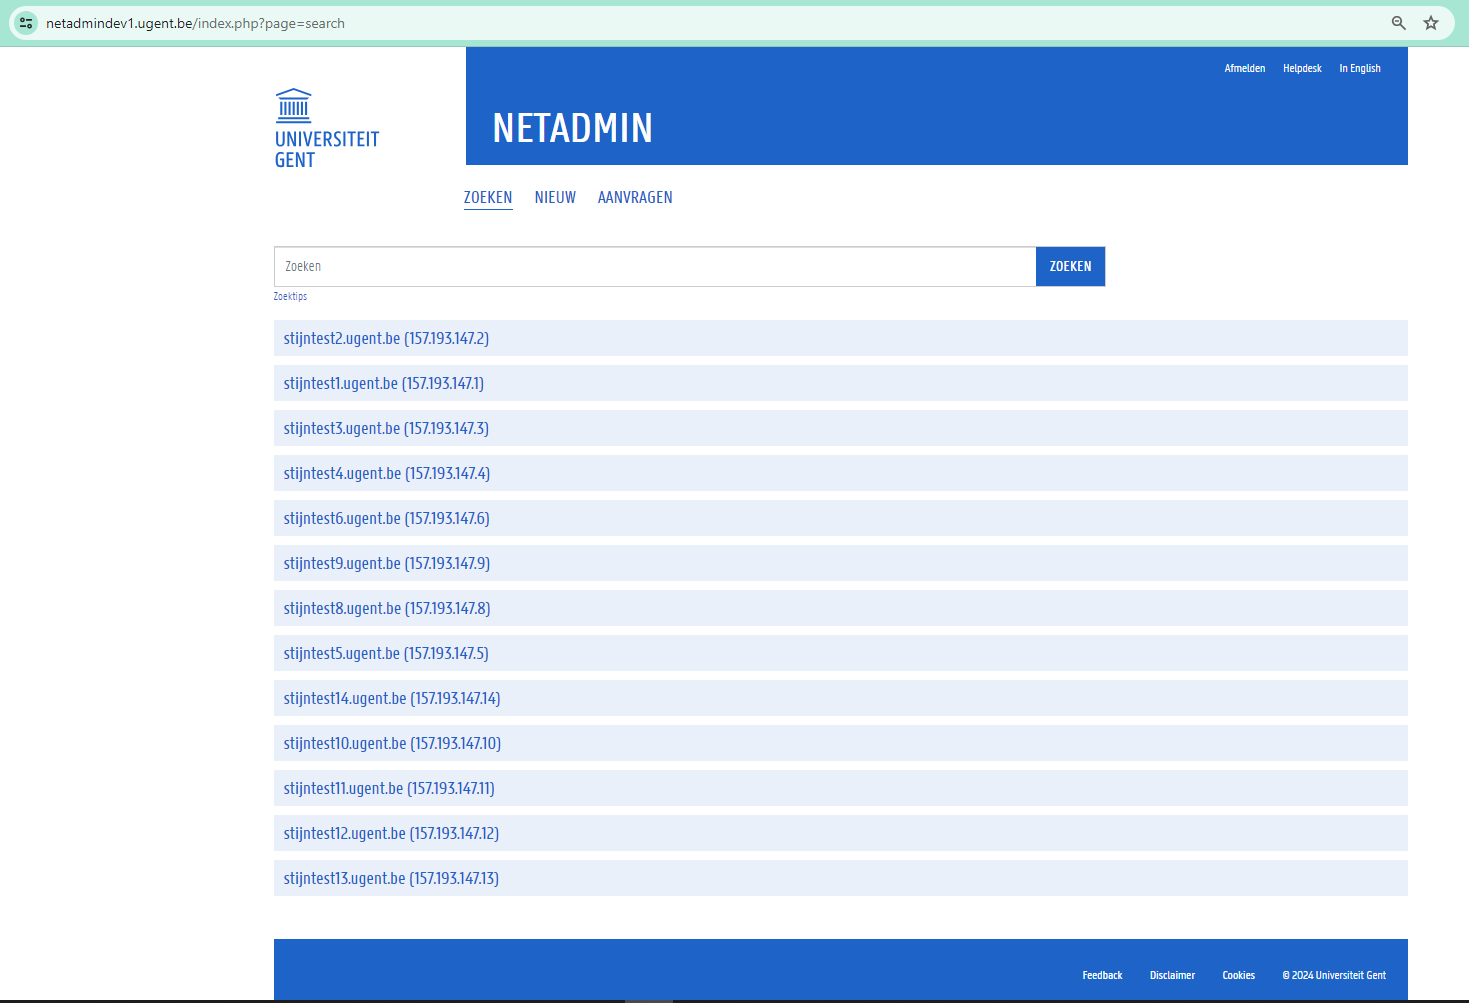
\includegraphics[width=15cm]{netadmin_ZoekHost_MeerdereHosts.png}
    \caption{Meerdere resultaten}
    \label{fig:netadmin_ZoekHost_MeerdereHosts}
\end{figure}
\begin{figure}[H]
    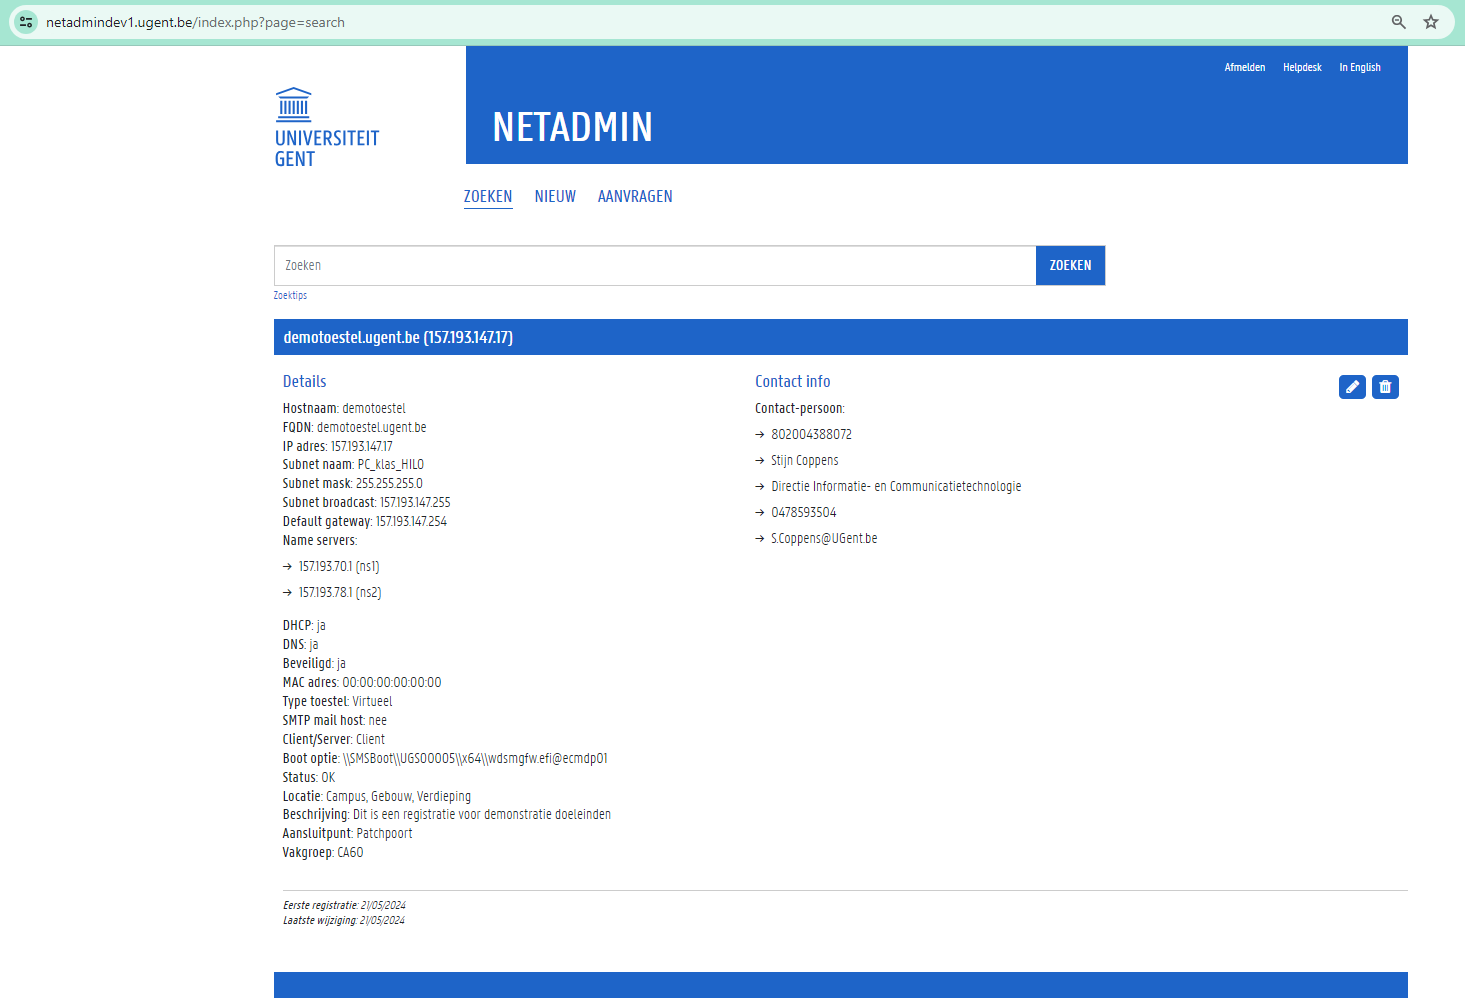
\includegraphics[width=15cm]{netadmin_ZoekHost_1host.png}
    \caption{Detail van een host}
    \label{fig:netadmin_ZoekHost_1host}
\end{figure}
\begin{figure}[H]
    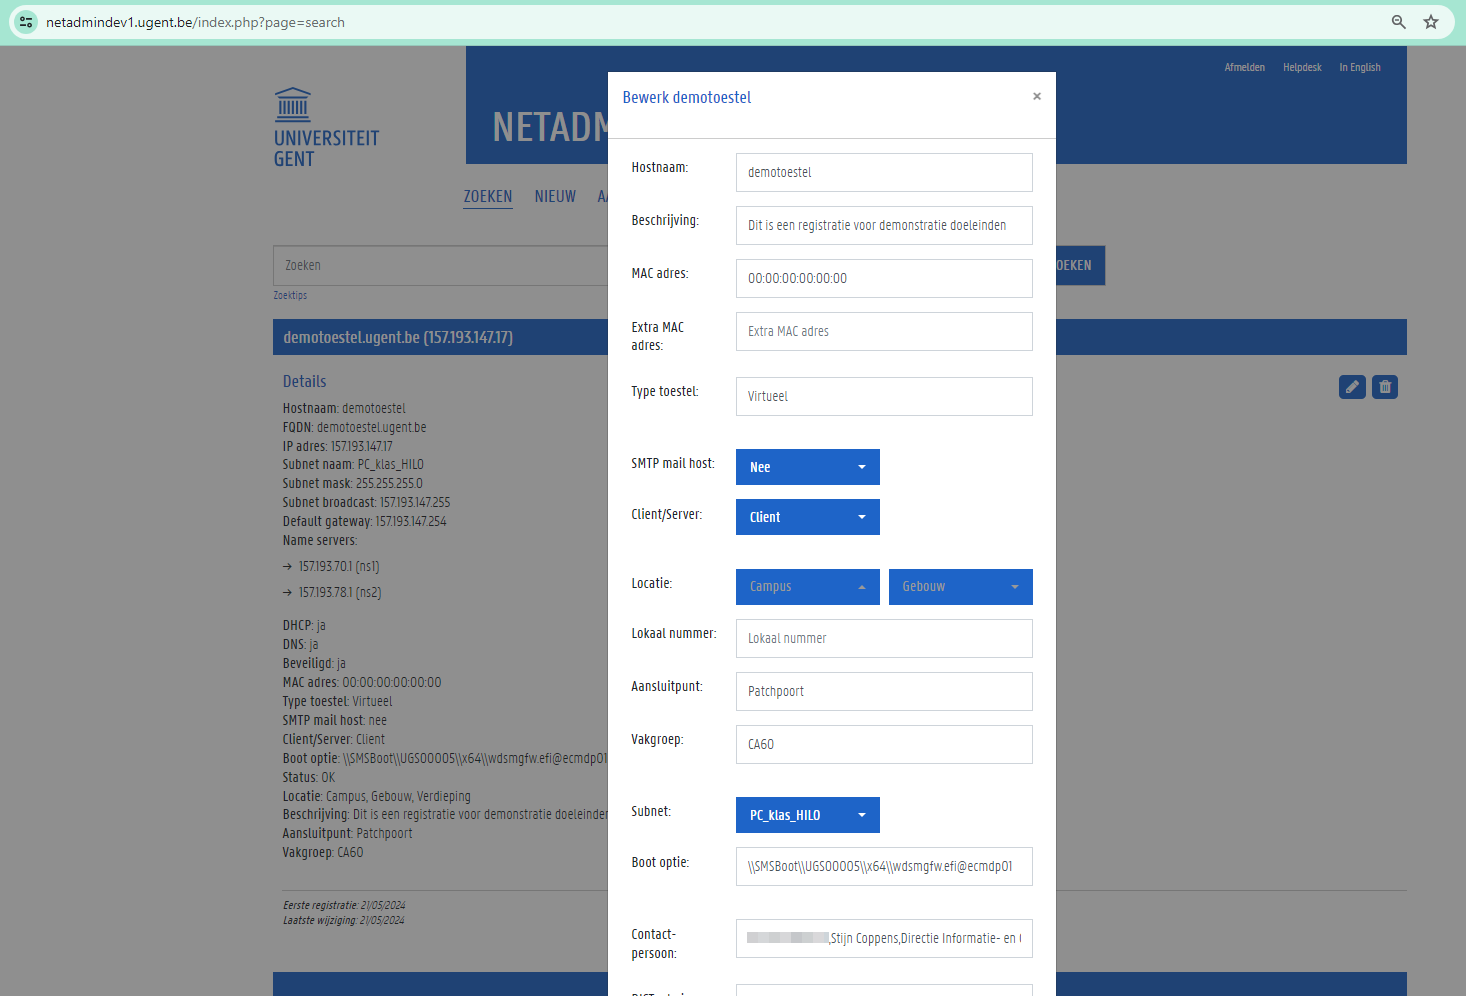
\includegraphics[width=15cm]{netadmin_ZoekHost_BewerkHost.png}
    \caption{Meerdere resultaten}
    \label{fig:netadmin_ZoekHost_BewerkHost}
\end{figure}
\subsection{Back-end}
Voor de back-end van deze pagina is het python-script \textit{getHosts.py} geschreven. Nadat alle nodige logging-acties genomen zijn, zal het script de meegegeven argumenten controleren  op aantallen en weggeschrijven naar een variabele. Hierna zal het script een configuratiebestand op de webserver uitlezen waarin onder andere de inloggegevens voor EfficientIP staan. Als dit allemaal correct verloopt, worden de inloggegevens voor EfficientIP opgehaald. Daarna wordt op basis van enkele functies beslist wat voor zoekterm is meegegeven als argument. Op basis van deze beslissing wordt dan contact gemaakt met EfficientIP via de juiste API-call. Naast de zoekterm kan het script ook één of meerdere vakgroepen als argument ontvangen. Als dit het geval is, worden deze vakgroepen gebruikt om de resultaten te filteren die de gebruiker kan opvragen. Op deze manier krijgt de gebruiker alleen resultaten te zien waarvoor die geautoriseerd is.

Indien EfficientIP antwoordt dat er geen registraties zijn op basis van de zoekterm, wordt dit weggeschreven in de log en eindigt het script. Indien EfficientIP wel registraties teruggeeft, wordt een onderscheid gemaakt op basis van het aantal registraties.
Indien er meer dan 1 registratie wordt weergegeven, wordt enkel de FQDN, IP, MAC en IP-ID van elke registratie in een lijst weggeschreven naar de output van het script. Als er maar 1 registratie is, wordt de host volledig verwerkt. Deze verwerking zal nog extra API-calls naar EfficientIP sturen om bijvoorbeeld de aliasen die tot de registratie behoren op te halen.

Deze aanpak is gekozen omdat sommige zoektermen, zoals vakgroep of campus, een groot aantal registraties kunnen opleveren, wat kan resulteren in een langere wachttijd voordat de gebruiker zijn resultaten te zien krijgt. Indien een gebruiker dan een registatie openklikt, zal het script nogmaals de host opzoeken op basis van IP-ID, waardoor die maar 1 resultaat zal moeten verwerken en weergeven.

\section{Pagina: Nieuwe registratie}
\label{nieuwe-registratie}
Deze pagina laat ingelogde gebruikers toe om nieuwe registraties te maken. De velden die worden weergegeven hangen af de gebruikersgroep uit sectie \ref{toegangsregels} waartoe de gebruiker behoort.

\subsection{Front-end}
Zoals weergegeven in figuur \ref{fig:netadmin_NieuweHost} wordt een formulier weergegeven waarbij bij sommige velden een keuze gemaakt moet worden op basis van een oplijsting. Indien meer informatie over een veld nodig is kan de gebruiker dit terugvinden door met de cursor over het veldnaam te zweven. Ook deze functie is zichtbaar in figuur \ref{fig:netadmin_NieuweHost}.
Een voorbeeld daarvan is locatie, waarbij de gebruiker een campus en gebouw moet kiezen. Eens deze gekozen zijn, zal achterliggend een script worden uitgevoerd dat op basis van de FI-code van het gebouw alle subnetnamen van subnetten ophaalt die in dat gebouw worden gebruikt. Deze lijst van subnetnamen wordt vervolgens gefilterd op basis van de gebruikersgroep waartoe de gebruiker behoort. Zo zal een gewone gebruiker enkel subnetnamen te zien krijgen met “data” of “colo” in de naam. De gebruiker kan dan het juiste subnet kiezen uit de gepresenteerde lijst zoals terug te vinden in figuur \ref{fig:netadmin_NieuweHost_oplijstingSubnets}. Indien de hostnaam reeds in gebruik is als hostnaam of alias, zal een gepaste foutmelding weergeven worden zoals in figuur \ref{fig:netadmin_NieuweHost_Foutmelding}. Als de vereiste velden ingevuld zijn en de hostnaam niet in gebruik is zal ook hier een gepaste melding weergegeven worden zoals te zien in figuur \ref{fig:netadmin_NieuweHost_SuccessRequest}.
\begin{figure}[H]
    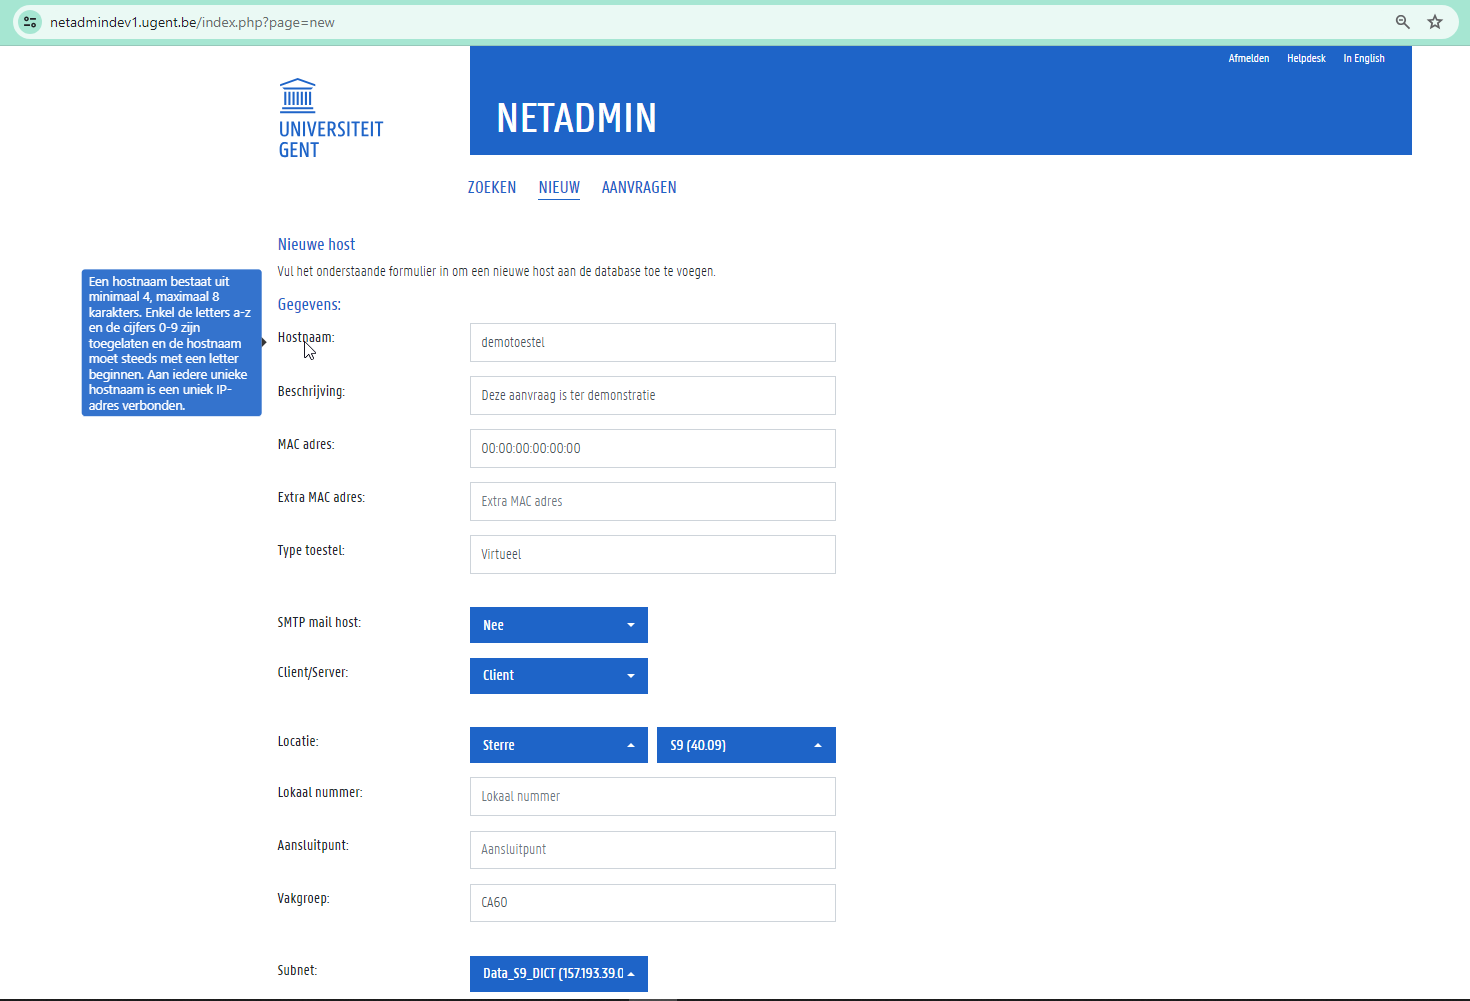
\includegraphics[width=15cm]{netadmin_NieuweHost.png}
    \caption{Meerdere resultaten}
    \label{fig:netadmin_NieuweHost}
\end{figure}
\begin{figure}[H]
    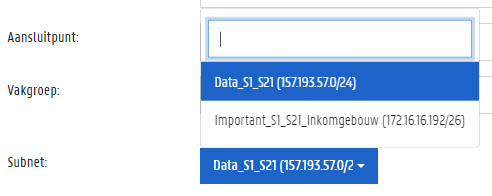
\includegraphics[width=10cm]{netadmin_NieuweHost_oplijstingSubnets.png}
    \caption{Oplijsting Subnetnamen}
    \label{fig:netadmin_NieuweHost_oplijstingSubnets}
\end{figure}
\begin{figure}[H]
    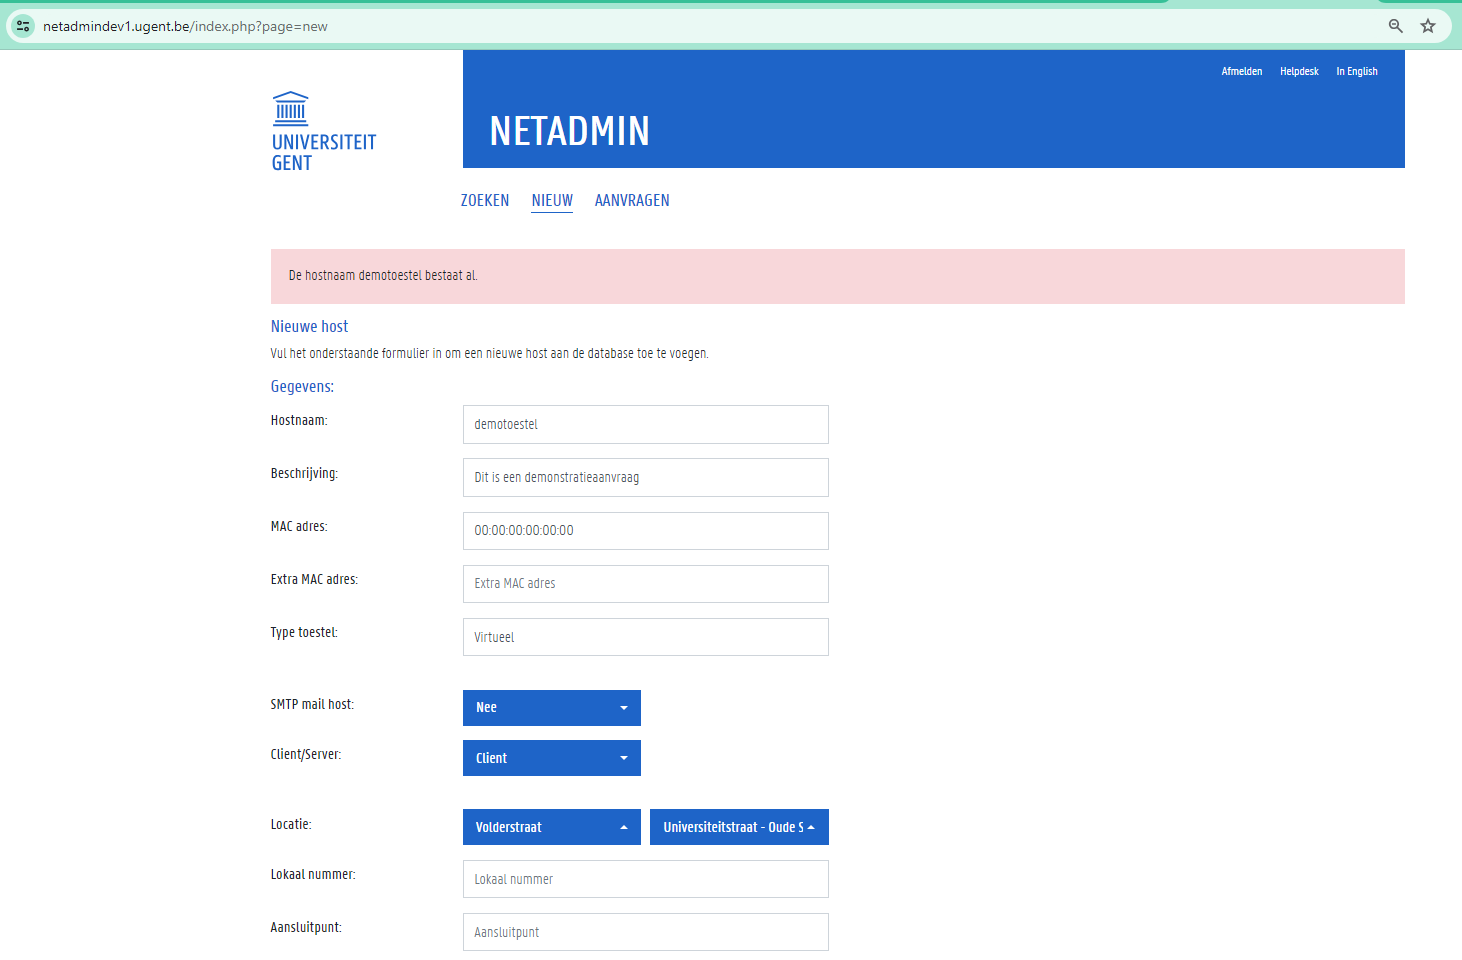
\includegraphics[width=15cm]{netadmin_NieuweHost_Foutmelding.png}
    \caption{Hostnaam foutmelding}
    \label{fig:netadmin_NieuweHost_Foutmelding}
\end{figure}
\begin{figure}[H]
    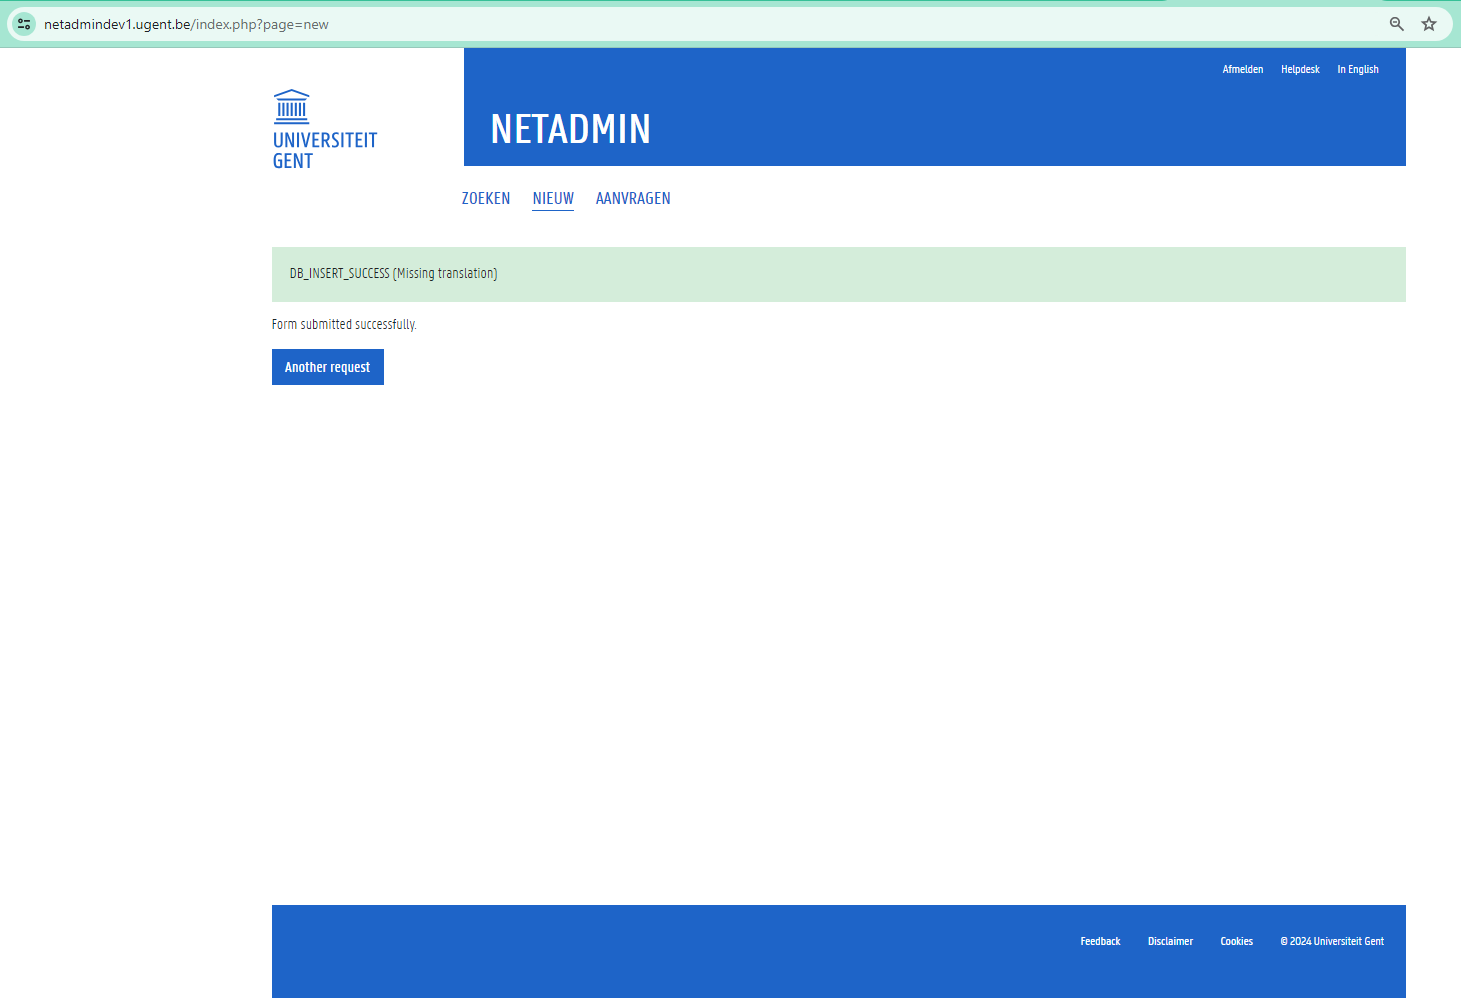
\includegraphics[width=15cm]{netadmin_NieuweHost_SuccessRequest.png}
    \caption{Succesvolle registratie}
    \label{fig:netadmin_NieuweHost_SuccessRequest}
\end{figure}
\subsection{Back-end}
Voor het ophalen van de subnetten op basis van FI-code is het python-script \textit{getSubnets.py} geschreven. Ook dit script schrijft een log weg, controleert de meegegeven argumenten op aantallen en leest het configuratiebestand op de webserver uit waarin onder andere de inloggegevens voor EfficientIP staan. Dit script accepteert twee argumenten: campus en gebouw. Op basis van een JSON-bestand waarin alle campussen en gebouwen en de daarbij horende FI-codes staan, wordt de juiste FI-code opgehaald. JSON (JavaScript Object Notation) is een lichtgewicht dataformaat dat gemakkelijk leesbaar is voor mensen en eenvoudig te parsen en te genereren is door machines. Daarna zal het script via een API-call alle subnetten die tot deze FI-code behoren, ophalen binnen EfficientIP. Voor elk subnet in de resultaten wordt de volgende informatie weggeschreven naar de output van het script:
\begin{itemize}
    \item \textbf{Name}: Naam van het subnet.
    \item \textbf{Mask}: Netwerkmasker van het subnet, hiervoor wordt een vertaling gedaan van de subnet grootte naar het netwerkmasker.
    \item \textbf{Broadcast}: Het broadcastadres van het subnet, dit is het laatste adres van het netwerk.
    \item \textbf{Address}: Dit is het eerste adres van het netwerk gevolgd door de prefix van het netwerk. Dit geeft een duidelijk beeld wat het bereik is van dit subnet.
    \item \textbf{ID}: Dit is het ID waaronder het subnet gekend is binnen EfficientIP.
    \item \textbf{Dot1x}: Hierin wordt weergegeven of dot1x actief is in dit subnet. IEEE 802.1X, oftewel Dot1x, actief is een netwerktoegangscontroleprotocol dat authenticatie regelt voor apparaten die verbinding maken met een netwerk, waarbij alleen geautoriseerde gebruikers toegang krijgen tot het netwerk. %TODO: BRON
    \item \textbf{Gateway}: Dit is de gateway van het subnet, het adres van de router die elke host binnen het netwerk moet gebruiken om buiten het netwerk te communiceren.
    \item \textbf{Subdomain}: Het eventuele DNS-subdomein binnen het UGent domein waartoe dit subnet behoort, indien er één is.
    \item \textbf{Nameservers}: Een oplijsting van de twee DNS-servers die binnen dit subnet gebruikt worden voor DNS-vertalingen.
    \item \textbf{Data}: Dit veld bevat True of False, naargelang of “\textit{data}” in de naam van het subnet zit.
    \item \textbf{Important}: Dit veld bevat True of False, naargelang of “\textit{important}” in de naam van het subnet zit.
    \item \textbf{Colo}: Dit veld bevat True of False, naargelang of “\textit{\_colo}” in de naam van het subnet zit.
\end{itemize}
Indien er geen subnetten zijn die tot de gevraagde FI-code behoren, zal dit in de log terecht komen en zal de gebruiker een gepaste melding krijgen.

\section{Pagina: Aanvragen}
\label{aanvragen}
Deze pagina, die exclusief voor de netwerkbeheerders is, wordt gebruikt om aanvragen bij te werken en goed of af te keuren.

\subsection{Front-end}
Op deze pagina is, zoals terug te vinden in figuur \ref{fig:netadmin_Aanvragen}, een overzicht van alle registraties te zien. In de MySQL-tabellen zijn bij elke registratie twee velden die aangeven wat de status van een registratie is:
\begin{itemize}
    \item \textbf{Approved}: Dit veld geeft via nummers weer wat de goedkeuringsstatus is van de registratie. Dit kan zijn 0 (wachtende), 1 (goedgekeurd), of 2 (afgekeurd).
    \item \textbf{Netadmin\_Handeld}: Dit veld geeft via nummers aan of de registratie in de database reeds gesynchroniseerd is met EfficientIP. Dit kan zijn 0 (nog niet verwerkt), of 1 (verwerkt).
\end{itemize} 
Deze pagina geeft een overzicht van alle registraties die nog niet goedgekeurd zijn door de netwerkbeheerders en die nog niet verwerkt zijn en dus nog niet op EfficientIP staan. Nieuwe registraties zullen nog geen IP-adres hebben, deze worden automatisch gevuld wanneer de netwerkbeheerders de pagina laden.
Netwerkbeheerders zullen hier registraties kunnen aanpassen, goedkeuren, afkeuren en, al dan niet, commentaar toevoegen. Via labels, zoals te zien aan de rechterzijde van elke registratie in figuur \ref{fig:netadmin_Aanvragen_MeerInfo}, is snel te zien of een registratie een opmerking bevat of een server registratie is. Indien op de registratie geklikt wordt zal de netwerkbeheerder meer informatie over de aanvraag zien.
\begin{figure}[H]
    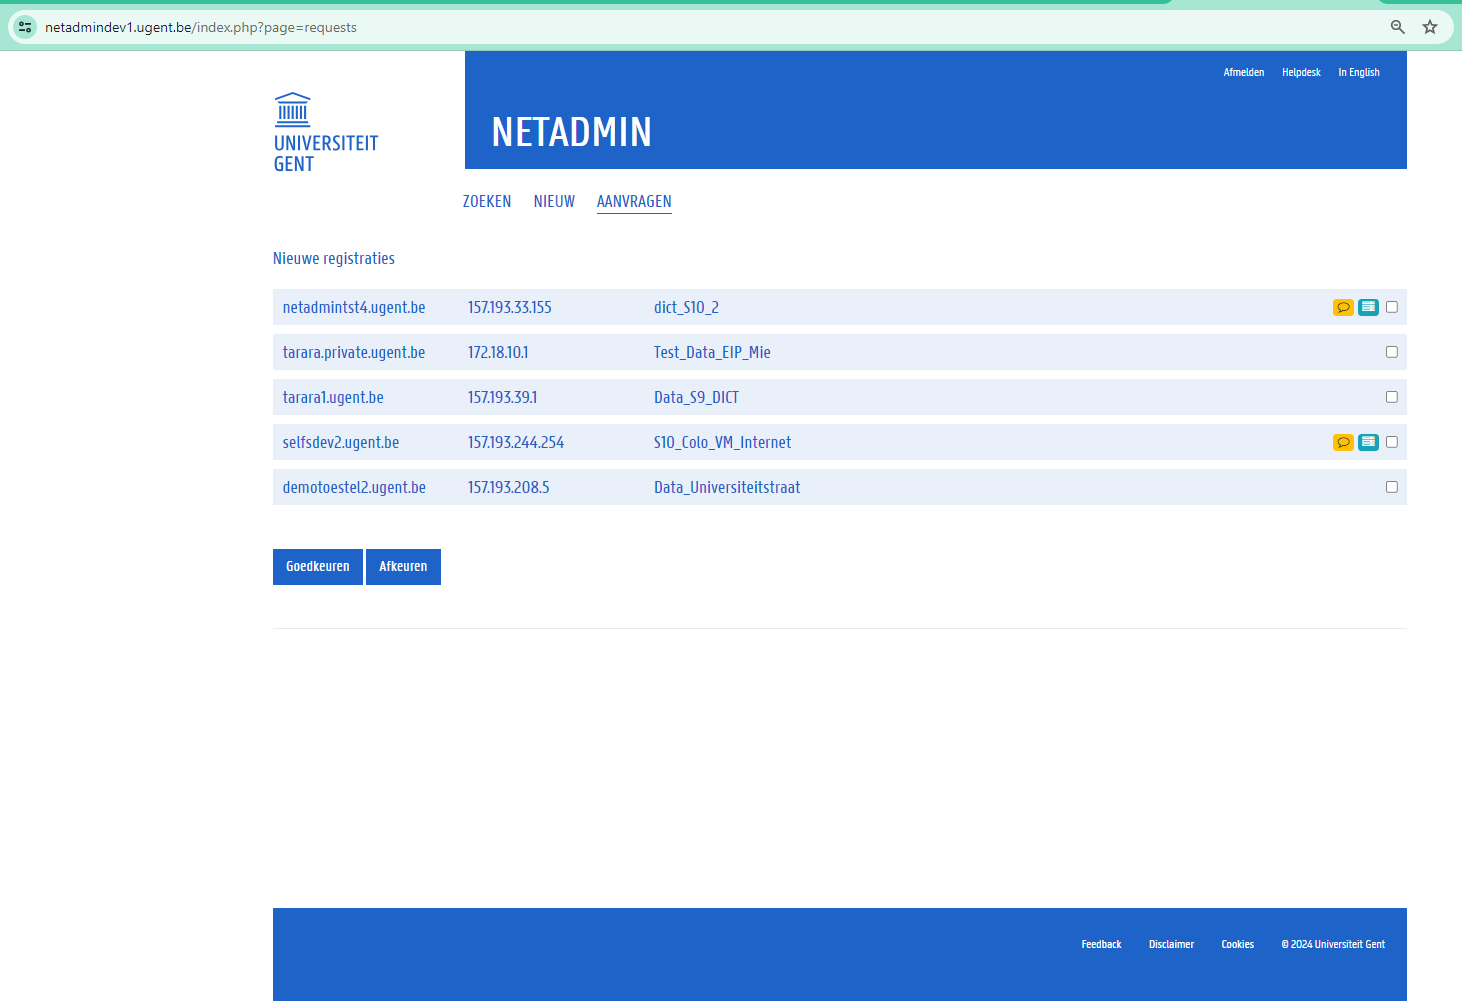
\includegraphics[width=15cm]{netadmin_Aanvragen.png}
    \caption{Overzicht netadmin aanvragen}
    \label{fig:netadmin_Aanvragen}
\end{figure}
\begin{figure}[H]
    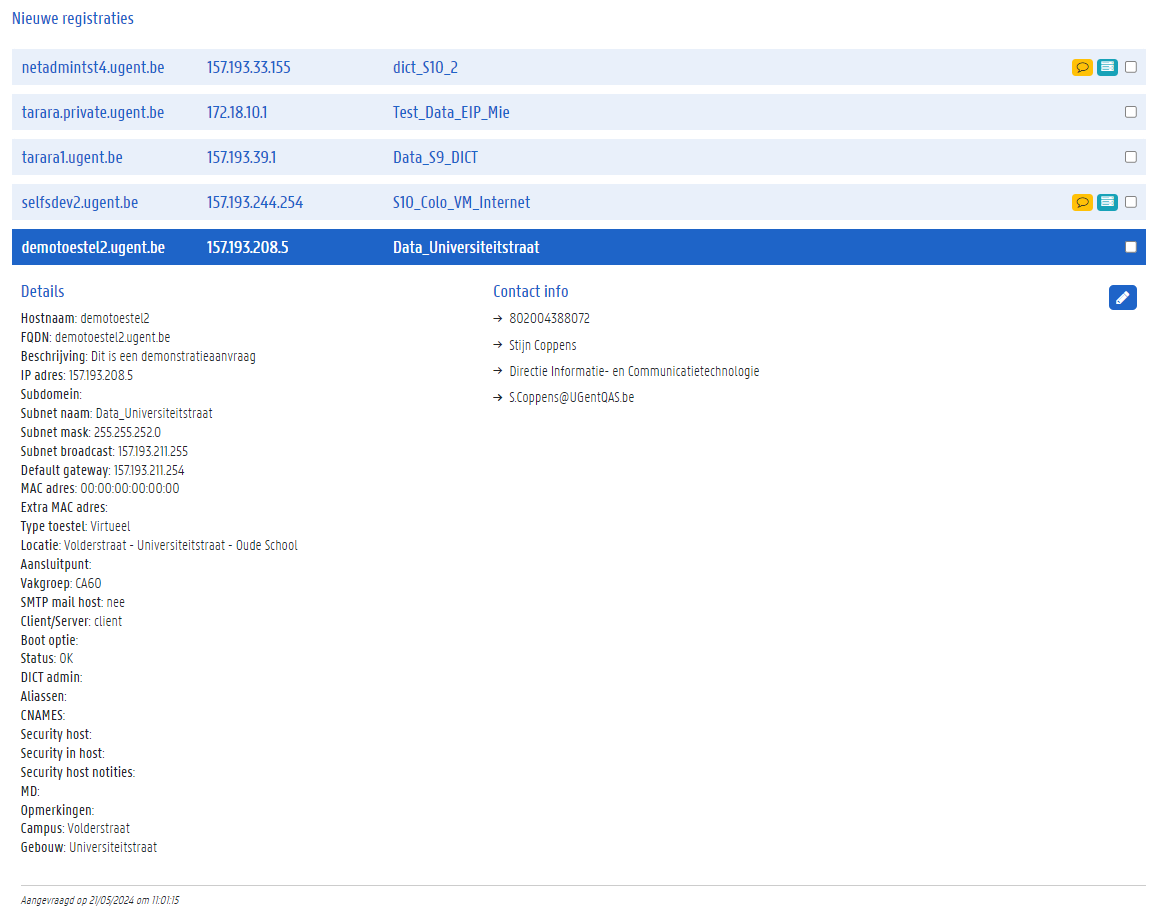
\includegraphics[width=15cm]{netadmin_Aanvragen_MeerInfo.png}
    \caption{Meer info van aanvraag registratie}
    \label{fig:netadmin_Aanvragen_MeerInfo}
\end{figure}
\subsection{Back-end}
Bij het laden van de aanvragen-pagina krijgen alle registraties die nog geen IP-adres in de database hebben, een IP-adres toegewezen voor het subnet waarin de registratie zich bevindt.
Netwerkbeheerders kunnen via een knop op deze pagina IP-adressen ophalen voor elke nieuwe registratie die nog geen IP-adres bevat.
Hiervoor wordt het python-script \textit{getAvailableIP.py} gebruikt. Dit script accepteert twee argumenten: het subnet-ID en dot1x. Dit is allebei info die wordt meegegeven bij het ophalen van elk subnet (zie back-end in sectie \ref{nieuwe-registratie}). Nadat de logging is ingesteld, het configuratiebestand inclusief de inloggegevens van EfficientIP en MySQL zijn gelezen en de argumenten zijn gecontroleerd, wordt er een API-call gemaakt naar EfficientIP op basis van het meegegeven subnetID. Als er geen beschikbare IP-adressen zijn, wordt dit gelogd en krijgt de netwerkbeheerder een melding dat die het subnet moet opschonen.
Indien er wel vrije IP-adressen in het subnet beschikbaar zijn, wordt er nagekeken of het IP-adres in een pool zit, wat voor pool dit is, of dot1x actief is en of het IP-adres al in gebruik is door een andere registratie en dus reeds is toegewezen in de MySQL tabel new\_hosts. Het script geeft tenslotte een lijst van beschikbare IP-adressen als output voor de front-end.

\section{Wijzigingen verwerken}
\label{wijzigingen-verwerken}
Er worden eveneens drie scripts geschreven die op de webserver geplaatst zullen worden en die periodiek zullen draaien.
Deze drie python-scripts zijn \textit{processNewHosts.py}, \textit{processChangeHosts.py} en \textit{processDeleteHosts.py}.

In tegenstelling tot de voorgaande scripts worden er geen argumenten meegegeven, deze scripts zetten logging op, lezen het configuratiebestand met onder andere de inloggegevens van EfficientIP uit en beginnen elk met het verwerken van alle goedgekeurde, onverwerkte registraties in de tabel die daarvoor voorzien is. Bijvoorbeeld processNewHosts.py kijkt in de database enkel naar de tabel new\_hosts.
Alle URL's die nodig zijn om de host aan te maken, te wijzigen of te verwijderen via een API-call worden per host in een lijst geplaatst.
Nadat alle URL's gemaakt zijn, wordt geteld hoeveel dit er zijn, en wordt gekeken of deze boven een bepaald getal uitkomen.
Dit getal is een zogenaamde \textit{fail-safe}. Indien er teveel URL's zijn, is er iets foutgelopen en wordt dit gelogd, en worden er dus geen API-calls gemaakt naar EfficientIP.
Als de fail-safe niet afgaat, worden alle URL's per hostregistratie afgegaan en naar EfficientIP verzonden. 
Indien elke call voor een registatie succesvol verloopt (dit weet het script op basis van het antwoord van EfficientIP), zal het script contact maken met de MySQL database en de waarde aanpassen om aan te geven dat de registratie verwerkt is.



